\documentclass[12pt, a4paper]{article}


% **************************************
% *            中文字体设置              *
% **************************************
\usepackage{xeCJK}
\usepackage[UTF8]{ctex}
\setmainfont{Times New Roman}
\setCJKmainfont{宋体}

\setCJKfamilyfont{zhhei}{黑体}
\newcommand*{\hei}{\CJKfamily{zhhei}}
\setCJKfamilyfont{zhkai}{楷体}
\newcommand*{\kai}{\CJKfamily{zhkai}}
\setCJKfamilyfont{enroman}{Times New Roman}
\newcommand*{\mytimes}{\CJKfamily{enroman}}

% **************************************
% *            页面设置                 *
% **************************************
\usepackage[left=2.0cm, right=2.0cm, top=2.0cm, bottom=2.0cm]{geometry} %设置页边距的宏包

\usepackage{graphicx} %插入图片的宏包
%\graphicspath{{chapter/}{figures/}}
\usepackage{indentfirst} %自动缩进
\usepackage{xcolor} %语法高亮支持
\usepackage{float} %可以用于禁止浮动体浮动
\usepackage{subfigure} %插入多图时用子图显示的宏包

\usepackage[colorlinks,linkcolor=black,anchorcolor=blue,citecolor=black]{hyperref}
\hypersetup{hidelinks} %隐藏超链接上的外框
%\usepackage[colorlinks,linkcolor=red]{hyperref}%超链接

\usepackage{fontspec,xltxtra,xunicode}
\defaultfontfeatures{Mapping=tex-text} %如果没有它,会有一些 tex 特殊字符无法正常使用,比如连字符
% 文章内中文自动换行,可以自行调节
\XeTeXlinebreaklocale “zh”
\XeTeXlinebreakskip = 0pt plus 1pt minus 0.1pt

% 下面的命令设置行间距与段落间距
\linespread{1.4}
% \setlength{\parskip}{1ex}
\setlength{\parskip}{0.5\baselineskip}

\usepackage{fancyhdr} %使用fancyhdr包自定义页眉页脚
%\pagestyle{empty}
\pagestyle{fancy}
%\pagestyle{plain} %没有页眉,页脚放页数
\renewcommand{\headrulewidth}{0.5pt}
\renewcommand{\footrulewidth}{0.4pt}
\lhead{}
\chead{}
\rhead{}
\lfoot{}
\cfoot{\thepage}
\rfoot{}
\usepackage{booktabs} %表格用


\usepackage{listings} %可以插入代码
%代码格式
\definecolor{dkgreen}{rgb}{0,0.6,0}
\definecolor{gray}{rgb}{0.5,0.5,0.5}
\definecolor{mauve}{rgb}{0.58,0,0.82}
\lstset{ %
	%	language=Python,                % the language of the code
	breaklines, %自动折行
	%extendedchars=false %解决代码跨页时,章节标题,页眉等汉字不显示的问题
	keepspaces=false,
	%tabsize=4 %设置tab空格数
	showspaces=false, %不显示空格
	showtabs=false,
	showstringspaces=true,
	numbers=left,
	basicstyle=\footnotesize,
	numberstyle=\tiny,
	numbersep=5pt,
	keywordstyle= \color{ blue!70}, %关键字颜色
	commentstyle= \color{red!50!green!50!blue!50}, %注释颜色 
	frame=shadowbox, %边框格式:阴影效果
	rulesepcolor= \color{ red!20!green!20!blue!20},
	escapeinside=``, %英文分号中可写入中文
	xleftmargin=2em,xrightmargin=2em, aboveskip=1em,  %设置页边距
	framexleftmargin=2em
}

% **************************************
% *      数学符号                       *
% **************************************
\usepackage{amsmath,amssymb}
\usepackage{bm} % $\bm{letter}$ 数学式中粗斜体字母的最佳方案
\usepackage{calc}
\usepackage{units} %单位宏包

% **************************************
% *     定义中文字号                     *
% **************************************
\newcommand{\chuhao}{\fontsize{42pt}{\baselineskip}\selectfont}
\newcommand{\xiaochuhao}{\fontsize{36pt}{\baselineskip}\selectfont}
\newcommand{\yihao}{\fontsize{28pt}{\baselineskip}\selectfont}
\newcommand{\erhao}{\fontsize{21pt}{\baselineskip}\selectfont}
\newcommand{\xiaoerhao}{\fontsize{18pt}{\baselineskip}\selectfont}
\newcommand{\sanhao}{\fontsize{15.75pt}{\baselineskip}\selectfont}
\newcommand{\sihao}{\fontsize{14pt}{\baselineskip}\selectfont}
\newcommand{\xiaosihao}{\fontsize{12pt}{\baselineskip}\selectfont}
\newcommand{\wuhao}{\fontsize{10.5pt}{\baselineskip}\selectfont}
\newcommand{\xiaowuhao}{\fontsize{9pt}{\baselineskip}\selectfont}
\newcommand{\liuhao}{\fontsize{7.875pt}{\baselineskip}\selectfont}
\newcommand{\qihao}{\fontsize{5.25pt}{\baselineskip}\selectfont}

% **************************************
% *     定义摘要、关键词、章节等命令        *
% **************************************
%%%% 设置 section 属性 %%%%
\makeatletter
\renewcommand\section{\@startsection{section}{1}{\z@}%
{-1.5ex \@plus -.5ex \@minus -.2ex}%
{.5ex \@plus .1ex}%
{\normalfont\sihao\bf\hei}}
\makeatother

%%%% 设置 subsection 属性 %%%%
\makeatletter
\renewcommand\subsection{\@startsection{subsection}{1}{\z@}%
{-1.25ex \@plus -.5ex \@minus -.2ex}%
{.4ex \@plus .1ex}%
{\normalfont\xiaosihao\bf\hei}}
\makeatother

%%%% 设置 subsubsection 属性 %%%%
\makeatletter
\renewcommand\subsubsection{\@startsection{subsubsection}{1}{\z@}%
{-1ex \@plus -.5ex \@minus -.2ex}%
{.3ex \@plus .1ex}%
{\normalfont\xiaosihao\hei}}
\makeatother

%%%% 段落首行缩进两个字 %%%%
\makeatletter
\let\@afterindentfalse\@afterindenttrue
\@afterindenttrue
\makeatother
\setlength{\parindent}{2em}  %中文缩进两个汉字位

% ************************************** %
\newenvironment{preface}{%
\thispagestyle{empty}
\begin{center}
	\textbf{\hei\sanhao{前言}}
\end{center}
\par
{\normalfont\xiaosihao}
}

\makeatletter
\renewcommand\abstract{%
\kai\textbf{\hei{摘要:}}
{\normalfont\xiaosihao\kai}}
\makeatother

\newenvironment{enabstract}

\makeatletter
\renewcommand\enabstract{%
\textbf{Abstract: }
{\normalfont\xiaosihao\mytimes}}
\makeatother

%%%% 设置 key words 属性 %%%%
\newenvironment{keys}

\makeatletter
\renewcommand\keys{%
\kai\textbf{\hei{关键词:}}
{\normalfont\xiaosihao\hei}}
\makeatother

\newenvironment{enkeys}

\makeatletter
\renewcommand\enkeys{%
\textbf{Key words: }
{\normalfont\xiaosihao\mytimes}}
\makeatother



\begin{document}
% **************************************
% *            封 面 部 分              *
% **************************************
\begin{titlepage}
	\centering
	\includegraphics[width=0.64\textwidth]{zjgs_logo.ai}\par
	\vspace{2cm}
	{\hei\fontsize{32}{4}\selectfont 人工智能前沿技术课程报告}\par
	\vspace{11cm}
	{\kai\huge 黄璞}\par
	\vspace{0.1cm}
	{\kai\LARGE 23020090090}\par
	\vfill
% Bottom of the page
	{\large \today\par}
\end{titlepage}

% **************************************
% *             前 言                  *
% **************************************
\begin{preface}
	此报告为作者学习了《人工智能前沿技术》课程后,对所学知识的凝练、总结以及与个人研究方向相结合的思考。
	在本报告中总结了图神经网络,人工智能硬件,量子人工智能这些新兴研究领域及其在机器学习中的核心知识点,阐述了相关理念和领域发展方向。
	报告起始于对图的基本概念及表示方法的详尽阐述,涵盖了无向图、有向图、加权图等多种类型,分析了节点中心性、连通性等重要特性,
	并突出了图数据结构在网络分析任务中的关键作用。在此基础上,重点介绍了图神经网络(GNNs)如何突破传统特征工程的局限,实现对复杂图形数据的高效建模与深度学习。
	进一步,针对不同层级的特征工程技术,我细致解析了节点层面、连接层面乃至全图层面的特征构建策略,
	如节点的中心性度量、集群系数、图小块统计等局部属性,以及全局统计指标和嵌入式表示学习。
	特别地,通过图嵌入表示学习的方法,我们可以自动获取到能够反映节点间关系的低维连续向量表示,从而为后续各类预测任务提供有力支持。
	此外,我还总结了人工智能硬件基础知识、发展的趋势和面临的挑战,
	以及量子计算为人工智能开辟的新前景,这些内容对于理解未来智能系统的发展潜力至关重要。
	最后,报告结合我个人的研究方向——伪造语音检测,展示了图注意力网络(如AASIST模型)在解决此类实际问题时的创新应用,
	通过对实验结果的分析和总结,论证了图神经网络在深度伪造识别等实际场景下的有效性和前瞻性。
\end{preface}


% **************************************
% *            目 录 生 成              *
% **************************************
\newpage
\pagenumbering{gobble} % 在目录部分禁用页码
\tableofcontents


% **************************************
% *            正 文 开 始              *
% **************************************
\newpage
\pagenumbering{arabic} %重置页码计数器,并切换到阿拉伯数字(默认设置)
\setcounter{page}{1} %重置页码从1开始计数

\section{图神经网络理论与应用}

\subsection{图的概念及基本表示}
在图论中,一个图(G)由节点(或称顶点,Vertices)和边(Edges)组成。
系统作为一个整体被表述为网络或图(N,E),其中N代表节点集合,E代表边集合。

\subsubsection{图的种类}
无向图:节点之间的连接没有方向性,例如友谊关系、互联网中的超链接等。其邻接矩阵是对称的,即Aij=Aji。
有向图:节点间的连接具有方向性,如通信网络、社交媒体中的关注关系等。对于有向图,可能存在强连通和弱连通的概念。强连通图意味着任意两个节点间都存在双向路径;而弱连通图则是在忽视边的方向时整个图是连通的。
加权图:无论是无向还是有向图,边都可以赋予权重,表示节点之间联系的强度,如合作关系强度、互联网中网页间的链接权重等。
自环图:节点可以与自身相连,形成自环或自回路。
多重图:允许同对节点间存在多条边的情况。
连接带权重的图:在实际应用中,通常会根据具体情境给每条边赋予权重,以体现不同连接的重要性。

\subsubsection{图的基本表示方法}
邻接矩阵:用矩阵形式表示节点间的连接关系,矩阵元素Aij非零表示节点i和节点j之间存在连接,且可以存储边的权重信息。
连接列表和邻接列表:另一种常见的图表示方式,适合于节点数量较大但稀疏度较高的图。

\subsubsection{图的连通性}
连通图:在无向图中,任何两个节点可以通过一系列边相互到达。
不连通图由多个连通分量组成,每个连通分量内部是连通的,但不同分量之间没有直接的连接路径。

\subsubsection{图在机器学习中的应用}
图机器学习主要应用于解决节点级别的任务(如节点分类)、边级别的任务(如链接预测)、以及图级别的任务(如图分类或生成)。通过自动学习节点嵌入(embedding),可以将复杂的图结构映射到低维空间,使得相似节点在嵌入空间中距离较近,从而服务于下游预测任务,如社交网络分析、蛋白质互作网络研究、推荐系统设计等。

\subsubsection{图神经网络(GNNs)}
图神经网络是一种能够处理图数据的深度学习模型,它能够在保持图结构不变的情况下进行特征学习,并用于完成多种预测任务,同时避免了传统机器学习中繁琐的人工特征工程。

\subsection{传统图机器学习与特征工程}
传统图机器学习与特征工程涉及如何设计并应用传统机器学习算法处理图数据问题。
由于图结构的特殊性,机器学习模型不能直接输入一整张图,它只能输入一个矩阵或向量,所以要把节点、连接、图表达成一个向量,将向量输入到机器学习模型中,
故而特征工程的设计十分重要,传统特征工程包括节点属性特征、连接特征、全图特征等的提取和构造方法。
这些方法虽然在复杂性和表达能力上有所限制,但为后续引入深度学习技术提供了有益启示。

\subsubsection{节点层面的特征工程}
节点层面的特征工程主要是针对节点层面的图数据挖掘任务。以节点分类的问题为例:输入某个节点的D维向量到机器学习算法中,输出的结果是该节点属于某一类的概率。
由已知的图结构信息去推测未知节点的类型,因为训练时用到了未标记节点的特征,所以属于半监督学习。
此时特征工程的目标是刻画节点在网络中的结构特征与位置属性,具体分为以下几种:
\par
(1)节点的度(Node degree)指一个节点的度是指与该节点直接相连(通过边连接)的其他节点数量。
节点的度越大,通常代表这个节点在网络中的连接性越强、影响力可能更大或者信息传递的能力更强。在社会网络分析中,高度数节点可以被视为中心节点或枢纽节点,它们对于网络整体的连通性和信息传播具有重要影响。
\par
(2)节点的中心性(Node centrality)是衡量网络中一个节点相对重要性或影响力的一系列量化指标。
不同的中心性度量方法从不同角度评估节点在网络中的核心地位。例如:
特征向量中心性(Eigenvector centrality),即如果一个节点的周围节点都很重要,则该节点就很重要。一个节点的重要度为周围节点重要度的和再乘以一个常数。可以将其视为一种递归的过程,这样的过程同样可以看成是求邻接矩阵的特征向量。
介数中心性(Betweenness centrality),基于这样的理念:在网络中,那些位于大量最短路径上的节点往往扮演着信息传递或流控制的关键角色。具体来说,介数中心性B(v)是指通过节点v的所有对其他节点的最短路径总数与所有可能的最短路径总数之比。换句话说,节点v的介数中心性表示的是在网络中所有其他节点对之间的最短路径中,有多少比例会经过节点v。
接近中心性(Closeness Centrality)反映了一个节点与网络中其他所有节点的平均距离。具体来说,一个节点的接近中心性定义为其到网络中所有其他节点最短路径长度的倒数之和。
\par
(3)集群系数(Clustering coefficient)用于衡量网络中节点的局部紧密程度。它量化了一个节点的邻居之间形成连接的程度,即一个节点的邻接点两两直接相连的概率。
\par
(4)图小块(Graphlets)是由有限数量节点构成的小规模子图,且这些子图在形态上互不相同。通过统计网络中不同类型的图小块的数量和分布情况,可以细致入微地分析和比较复杂网络的局部特征。
具体来说,给定一个大小为k的节点集,其所有可能形成的非同构子图构成了k阶图小块集合。例如,对于3阶图小块,存在7种不同的形态,包括:自我环、线段、三角形以及几种更复杂的三节点连接方式。
\par

\subsubsection{连接层面的特征工程}
“Link-Level Prediction” ,也就是通过已知连接去补全未知连接,需要做的是将每一种连接编译成向量输入到机器学习算法当中。分为两种情况:
第一种情况是客观静态图,例如蛋白质、分子等客观存在的物质。
第二种情况是随时间变化的,例如论文引用量,社交网络等。
不管怎样都需要先提取连接的特征,将连接转变成D维向量,再输入到机器学习模型当中去进行打分,并从高到低降序排序,选出最高 n个连接预测结果。连接的特征可以分为三类:基于两节点距离;基于两节点局部连接信息;基于两节点在全图的连接信息。
\par
(1)基于两节点距离的特征
最短路径长度:表示两个节点之间最短路径上的边数,反映它们在拓扑结构上的直接或间接接近程度。
平均路径长度:通过计算所有节点对之间的平均最短路径长度来衡量整个网络的信息传播效率或者整体紧密程度。
\par
(2)基于两节点局部连接信息的特征
共享邻居计数:统计两个节点共享的邻接节点数量,可以反映节点间的相关性或社区结构属性。
局部聚类系数:评估一个节点及其相邻节点构成的子图内三角形的数量,作为局部密集连通性的指标。
本地中心性指标:如点度中心性、局部介数中心性等,这些只考虑节点的直接邻居关系,而不涉及更广泛的网络结构。
\par
(3)基于两节点在全图的连接信息的特征
全局中心性指标:如全局介数中心性、特征向量中心性等,这些指标不仅考察节点自身的连接情况,还关注节点在整个网络中扮演的中介作用和重要性。
社区结构信息:分析节点是否属于同一社团(社区)以及社团内部的连接强度,这可以帮助理解节点在整个网络中的角色和功能定位。
高阶图小块统计:通过统计两个节点参与的高阶图小块结构,可以获取更为复杂的拓扑关联信息。
\par

\subsubsection{全图层面的特征工程}
全图层面的特征工程是指从整个网络全局的角度提取和构建反映网络整体结构、特性及功能的特征。其核心理念是将整张图转变成D维向量,且该向量能够反应全图的结构特点。
以下是一些常见的全图层面特征工程方法:
\par
(1)全局网络统计量。如:
平均路径长度:所有节点对之间的平均最短路径长度,反映网络的信息传播效率。
聚类系数:评估网络中三角形出现的程度,揭示网络的集群性或社区结构。
边度分布、节点度分布:描述网络中边和节点数量分布的统计特性。
\par
(2)网络密度,指网络中的实际连接数与最大可能连接数的比例,用来衡量网络的整体连通程度。
\par
(3)中心性指标。如:
全局度中心性:所有节点度值的排序统计信息。
全局介数中心性:各节点在整个网络中作为桥梁的重要性度量。
全局特征向量中心性:通过计算网络的拉普拉斯矩阵特征向量,得到节点在整个网络中的影响力排名。
\par

\subsection{图嵌入表示学习}
受传统人工设计特征也就是特征工程去实现嵌入启发,我们也可以通过自监督或图表示学习的方法去实现嵌入。
核心问题也就是在保持图中节点或边之间关系的同时,如何把节点映射成D维向量。人工特征工程告诉我们,可以通过节点的中心性,集群系数以及图小块进行映射,而图表示学习则可以通过随机游走构造子监督学习任务。

\subsubsection{图嵌入定义}
图表示学习可以自动学习特征,把人工设计特征的步骤替换成表示学习。表示学习的定义是自动学习特征并将各模态输入转为向量。在图表示学习的过程中,每一个步骤都是全自动的,是端到端的,不需要人为干预。图表示学习避免了做特征工程的工作。
\par
图嵌入的过程就是将节点映射成D维向量,且映射出来的D维向量是低维、连续且稠密的,并且该D维向量与下游任务无关,我们并不关心下游任务是什么。故而这一过程中是无监督的。
D维向量应当有以下几个特征:
(1)两个节点的D维向量相似度反应出节点相似度。
(2)嵌入向量包含网络信息。虽然d维向量与下游任务无关,但是它所包含的信息足以解决下游任务。
\par

\subsubsection{图嵌入方法}
(1)编码器—解码器(Encoder-Decoder)架构
\par
编码器输入一个节点,输出一个D维向量,即把节点嵌入(映射)到D维空间中;
解码器输入D维空间中的向量,输出向量的相似度,进而能够反映节点的相似度。节点相似度需要人为定义,如可定义为余弦相似度。
\par
(2)基于随机游走的图嵌入方法
\par
随机游走即从A节点出发到B节点,可能会随机选择自己的下一个路线,同一个节点可能会出现很多次。每一个到达B点的过程都是一个随机游走的序列。
\par
DeepWalk是一种全随机的随机游走,思想是如果A节点和B节点出现在一个随机游走序列中,我们希望这个概率高,如果没有出现在同一随机游走序列中我们希望这个概率低。
如果两个节点出现在同一随机游走序列当中,则称这两个节点是相似的,这两个节点的向量积也会比较大。算法过程为:
\par
1)采样得到若干随机游走序列,计算条件概率
\par
2)迭代优化每个节点的D维向量,使得序列当中共现节点的条件概率大,不共现的数量积小。
\par
Node2Vec是一种有偏的二阶随机游走,通过控制P,Q两个超参数,控制一个游走处于它目前所在地区的领域还是让它更探索远端。

\subsection{半监督节点分类}
半监督节点分类是机器学习和图神经网络领域中的一个关键任务,它旨在利用有限的有标签数据以及大量未标记数据来预测整个图中所有节点的类别。在实际应用中,如社交网络分析、推荐系统、生物信息学等领域,获取大规模数据集的所有标签往往成本高昂或不可能实现,因此半监督学习方法就显得尤为重要。
在图数据中,节点之间的连接关系提供了额外的信息来源,这使得我们可以利用结构信息辅助分类过程。常用的半监督节点分类技术包括:
\par
(1)标签传播(Label Propagation):基于邻居节点的标签信息迭代地更新目标节点的标签,通过网络中信息的扩散来推测未标记节点的类别。
\par
(2)图卷积神经网络(Graph Convolutional Networks, GCNs):设计特定的卷积操作处理图数据,允许特征信息在网络上传播并融合,从而学习到每个节点的嵌入表示,并基于这些表示进行节点分类。
\par
(3)深度Walk-based方法:例如DeepWalk和Node2Vec等算法先通过随机游走生成节点序列,然后利用自然语言处理中的词嵌入技术(如Skip-gram模型)得到节点的低维向量表示,最后使用这些嵌入向量进行节点分类。
\par
(4)半监督消息传递机制:在GNNs框架下,节点通过接收和发送消息的方式与邻居节点交互,在多层神经网络结构中逐步整合全局和局部信息以完成节点表征的学习。
\par
拓扑不平衡学习:针对图上节点类别数量不均衡的问题,发展出相应的策略优化模型训练,确保不同类别的节点都能得到充分的学习和识别。
在评估阶段,通常会采用交叉熵误差度量有标签节点上的分类性能,并利用验证集对模型参数进行调整。最终的目标是在尽可能少的标注数据下获得准确率较高的节点分类结果。
\par

\section{人工智能硬件发展与挑战}
人工智能硬件发展是当前AI领域的重要趋势,它与传统的计算硬件不同,专门针对机器学习和深度学习算法的计算需求进行了优化。

\subsection{发展趋势}
\par
(1)专用芯片(ASICs):例如Google的TPU(张量处理单元),针对特定类型的神经网络运算进行高度优化,提供比通用处理器GPU或CPU更高的能效比。
\par
(2)FPGA和CGRA:可编程逻辑器件如现场可编程门阵列(FPGA)和可重构计算架构(CGRA) 能够灵活适应多种AI算法,同时提供较高的性能和较低的能耗。
\par
(3)边缘计算硬件:随着物联网的发展,越来越多的智能设备需要在本地实现一定程度的人工智能处理,因此轻量级、低功耗且高效的边缘计算硬件成为研发重点。
\par
(4)异构计算系统:结合CPU、GPU、TPU等多种计算单元构建高性能计算机集群,以应对大规模数据处理和训练任务。
\par

\subsection{面临的挑战}
\par
(1)算力要求:AI应用对计算能力的需求不断增长,尤其是对于复杂的深度学习模型,这要求硬件具备极高的并行处理能力和浮点运算速度。
\par
(2)能效比:尽管计算能力增强,但能耗问题仍然突出,特别是在移动设备和物联网场景下,需要提高单位能耗下的计算效率。
\par
(3)兼容性和标准化:各种定制化AI芯片的出现导致软件开发和部署的复杂性增加,缺乏统一的标准和接口可能导致生态系统碎片化。
\par
(4)隐私保护与安全:硬件层面如何保证数据安全传输、存储和计算过程中的隐私保护也是一个重要挑战。
\par
(5)成本与规模化生产:高端AI硬件的研发和制造成本高昂,如何降低生产成本以便于更广泛的应用是一个现实问题。
\par

\section{量子人工智能基础与前景}

\subsection{量子人工智能基础}
量子人工智能(Quantum Artificial Intelligence,QAI)是一个结合了量子计算和传统人工智能的新兴领域,主要基于以下几个方面:
\par
(1)量子计算基础:量子计算机利用量子比特(qubits)代替经典比特,并通过叠加态和纠缠态实现并行计算。量子算法如Shor's算法用于快速分解大质数、Grover搜索算法用于优化搜索过程等,为量子人工智能提供了强大的计算能力。
\par
(2)量子机器学习:借鉴经典机器学习原理,研究者正在开发基于量子计算机的机器学习模型和算法。这些方法包括但不限于量子神经网络(Quantum Neural Networks, QNNs)、量子支持向量机(Quantum Support Vector Machines, QSVMs)、以及量子强化学习(Quantum Reinforcement Learning, QRL)等。
\par
(3)量子优化:由于量子系统能够天然处理高维度空间问题,因此在解决复杂优化问题时具有潜力,这对于训练复杂的深度学习模型或解决组合优化问题至关重要。
\par
(4)量子数据处理与特征提取:量子计算可以用来处理大规模且高度结构化的数据集,尤其是在图数据和化学分子表示等领域,通过量子图嵌入或其他方法将非结构化数据转化为适合量子计算机处理的形式。
\par

\subsection{量子人工智能前景}
\par
(1)计算效率提升:理论上,量子计算能够在特定问题上提供指数级加速,这使得处理当前经典计算机难以解决的大规模机器学习任务成为可能。
\par
(2)新模型探索:量子机器学习不仅可能改进现有算法性能,也可能启发全新的学习模型和范式,尤其是在量子控制、量子通信和量子传感等方面的应用。
\par
(3)实际应用:虽然量子计算机目前仍处于发展阶段,但随着技术的进步,量子人工智能有望在未来应用于药物发现、金融分析、气候模拟、密码学等领域。
\par

\section{课程内容与个人研究方向结合的思考}

\subsection{个人研究方向——伪造语音检测}

相比传统的身份认证,生物身份认证被认为是一种更加便捷有效的认证方案,这是由于生物的身份信息蕴含于自身且独一无二,因此不存在
遗失的风险且不容易更改。声纹认证作为一种生物认证方式被越来越广泛地应用,如门禁、银行等。
同时,由于互联网的飞速发展,用户的信息非常容易泄露,导致犯罪分子在获取用户的语音信息后,利用合成技术进行语音诈骗,威胁人们的财产安全。
因此,研究有效的语音反欺骗技术和深度伪造语音检测技术至关重要。
\par

\subsubsection{传统的伪造语音检测技术}
传统的伪造语音检测技术\cite{魏为民}大多基于前端-后端(FrontEnd-BackEnd)框架,前端主要用于先提取语音信息特征,后端则针对语音信息特征建立分类器。
前端的特征提取包括频谱信息、相位特征、倒谱系数特征、动态声学特征等。后端的分类器包括支持向量机(SVM)和高斯混合模型(GMM)等。

\subsubsection{基于深度学习的端到端伪造语音检测技术}
随着深度学习的发展,深度神经网络在语音领域的应用也越来越广泛,
基于端到端的深度卷积神经网络被证明在伪造语音检测上取得了很好的效果。
但目前仍面临许多难题:
\par
(1)高度真实性和多样性:合成语音算法同样受益于深度学习技术的发展,伪造的语音能够达到非常高的逼真度,
甚至可以模拟说话者的情绪、语调和特定口音;合成算法层出不穷,不同的算法合成出的语音所产生的与真实语音的差异性存在于语音特征的各个不同区域。
这使得伪造语音检测模型需要非常良好的泛化性能,才能应对不同的合成算法。
\par
(2)缺乏通用特征:尚未发现一种适用于所有情况的稳定声纹特征或深度伪造痕迹,因此需要不断开发和优化用于识别伪造的声学特征提取方法。
\par
(3)对抗攻击:伪造者可能会利用对抗样本生成技术有意地制造难以被现有检测系统识破的伪造语音。
\par
(4)数据集不足:构建有效的语音伪造检测系统通常需要大量的真实语音和伪造语音样本进行训练,而大规模高质量的伪造语音数据往往不易获取。


\subsection{图注意力网络在伪造语音检测的应用}

最近的研究表明\cite{J. Yang},鉴别信息(语音合成算法的区分性特征)可以同时存在于频域和时域中,鉴别信息往往取决于攻击的性质和使用的具体算法。
之前的伪造语音检测单模型缺少同时关注频域和时域的鉴别信息,导致效果不佳,往往集成多个模型,每个模型关注不同的鉴别信息,但最终的效果会受到多模型后端分数融合时带来的对性能的影响。
AASIST 寻求开发一个高效、单一的系统,可以在没有分数级集合的情况下检测广泛的不同欺骗攻击,它一种新颖的异构堆叠图注意力层,该层通过异构注意力机制和堆叠节点对跨越异构时域和频域的鉴别信息进行建模。

\subsubsection{AASIST模型}

AASIST模型\cite{J. Jung AASIST}如图\ref{fig:AASIST-Framework}所示。
它主要主成部分包括RawNet2的编码器\cite{J. Jung RawNet2}、图模块(Graph module)、异构堆叠图注意力(Heterogeneous Stacking Graph Attention Layer, HS-GAL)、读出层(readout)组成。

\begin{figure}[htbp] % 使用浮动体环境来定位图片
	\centering % 使图片居中
	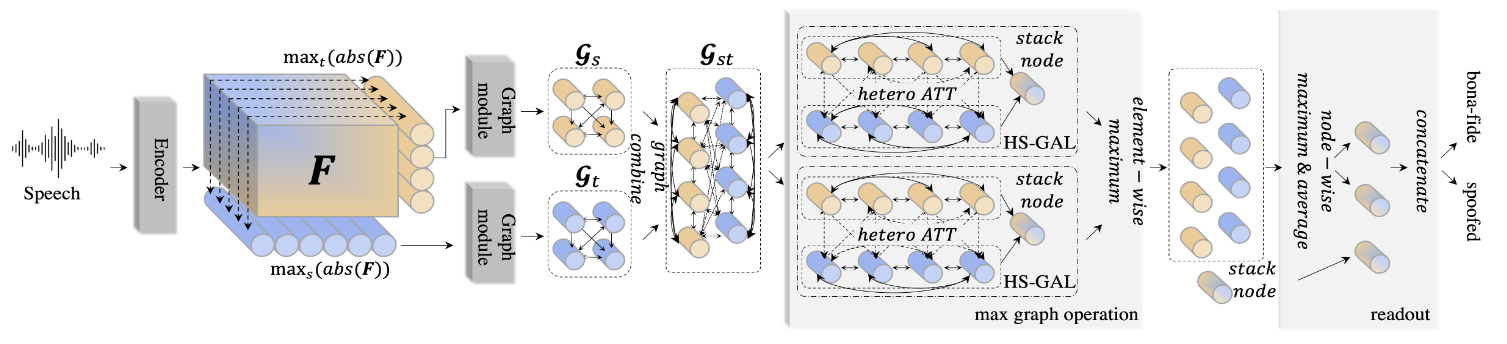
\includegraphics[width=0.9\textwidth]{AASIST-Framework.png} % 设置图片宽度为文本宽度的90%
	\caption{AASIST模型} % 图片标题
	\label{fig:AASIST-Framework} % 给图片添加标签以供引用
\end{figure}

RawNet2的编码器直接从原始语音波形输入中提取高级表示$F, F \in R^{C \times S \times T}$,其中$R, S, T$分别代表通道数,频谱间隔,时间序列长度。
图模块由图注意力网络(GAT)和图池化网络(Graph pooling)组成。两个图模块分别从域和频域两个方向处理高级表示$F$,使得它们可以同时关注不同的鉴别信息。
\par
Graph combination操作使得两个异构图进行结合,并输入到HS-GAL层中。
\par
HS-GAL的输入首先被投影到另一个隐空间中,使得节点维数为$D_t$和$D_s$的两个图中的每一个具有共同的维数$D_{st}$。为此使用了两个全连接层,每个全连接层将一个组成子图投影到$D_{st}$的一个维度。
HS-GAL中的异构注意力使用三个不同的投影向量来计算异构图的注意力权重。它们显示在图\ref{fig:AASIST-Framework}的$G_{st}$中,并用于确定连接边的注意力权重:
(1)$G_s$中的节点到$G_s$(橙色节点之间的边)中的节点;
(2) $G_s$到$G_t$和$G_t$到$G_s$的节点(点状边);
(3)$G_T$到$G_T$(蓝色节点之间的边)。
栈节点(Stack node)的作用是积累异质信息,即谱域和时域之间的信息或关系。
\par
最后读出层输出节点的最大值和平均值,最后一个隐藏层是由使用平均值和最大值得到的两个节点与堆栈节点级联形成的。

\subsubsection{实验结果分析}

论文实验结果如图\ref{fig:Results}所示。

\begin{figure}[htbp] % 使用浮动体环境来定位图片
	\centering % 使图片居中
	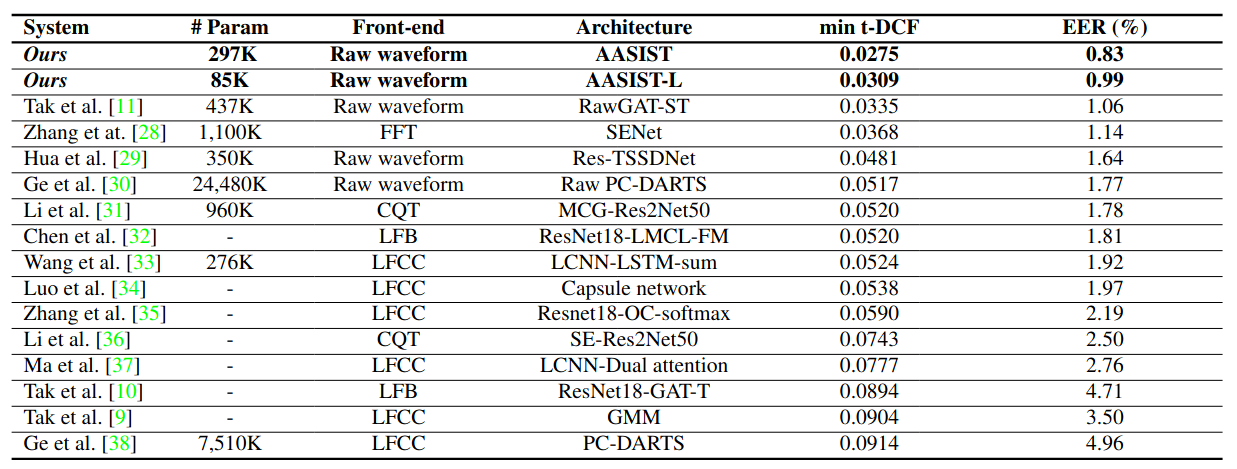
\includegraphics[width=0.9\textwidth]{Results.png} % 设置图片宽度为文本宽度的90%
	\caption{AASIST实验结果\cite{J. Jung AASIST}} % 图片标题
	\label{fig:Results} % 给图片添加标签以供引用
\end{figure}

可以看到,该论文与最近提出的最先进系统进行比较,使用 min t-DCF 和 EER 作为性能评价指标\cite{M. Todisco}。
结果使用 min t-DCF 以升序排列显示,图中所有的结果都是单一模型的表现,论文提出的 AASIST 和 AASIST-L(轻量化的AASIST),达到了最好的单一模型结果。

\subsubsection{总结与思考}

AASIST模型的核心是图注意力机制,与传统注意力机制相比,每个节点可以有任意数量和类型的邻居节点,
而且允许模型根据节点之间的关系动态地分配注意力权重,这意味着模型能够捕捉到图中任意两个节点间的复杂相互影响。
当它分别应用在语音的频域和时域时,它能够更容易捕捉到跨时间和跨子带中的信息关系,而语音合成算法产生的伪造语音所携带的鉴别信息就存在于这些地方。
这可能也是AASIST的性能为什么如此显著的原因。

\begin{thebibliography}{4}
	\bibitem{J. Yang}J. Yang, R. K. Das and H. Li, “Significance of subband features for synthetic speech detection,” IEEE Transactions on Information Forensics and Security, vol. 15, 2019.
	\bibitem{J. Jung AASIST}J. Jung, H. Heo, et al., “AASIST: Audio Anti-Spoofing using Integrated Spectro-Temporal Graph Attention Networks,” in Proc. ICASSP (to appear), 2022.
	\bibitem{J. Jung RawNet2}J. Jung, S. Kim, H. Shim et al., “Improved RawNet with Feature Map Scaling for Text-Independent Speaker Verification Using Raw Waveforms,” in Proc. Interspeech, 2020.
	\bibitem{M. Todisco}M. Todisco, X. Wang, V. Vestman et al., “Asvspoof 2019: Future horizons in spoofed and fake audio detection,” in Proc. Interspeech, 2019.
    \bibitem{魏为民} 魏为民,刘畅,才智等.合成语音检测方法的研究现状及展望[J].上海电力大学学报,2022,38(01):75-81.
\end{thebibliography}


\end{document}
